% Created 2021-09-05 nie 17:17
% Intended LaTeX compiler: pdflatex
\documentclass[11pt]{report}
\usepackage[utf8]{inputenc}
\usepackage[T1]{fontenc}
\usepackage{graphicx}
\usepackage[dvipsnames]{xcolor}
\usepackage{booktabs}
\usepackage{grffile}
\usepackage{longtable}
\usepackage{wrapfig}
\usepackage{rotating}
\usepackage[normalem]{ulem}
\usepackage{amsmath}
\usepackage{textcomp}
\usepackage{amssymb}
\usepackage{capt-of}
\usepackage{hyperref}
\usepackage{titlesec}
\usepackage{booktabs}
\usepackage{graphicx}
\usepackage{caption} 
\usepackage{subcaption} % for the subfloat in the figs
\usepackage{multirow}
%\usepackage{algorithm}
%\usepackage[noend]{algorithmic}
\usepackage{xspace}
\usepackage{epsfig}
\usepackage{amsmath}
\usepackage{amsthm}
\usepackage{amssymb}
\usepackage{times}
\usepackage{xr}

\newcommand{\V}{\mathcal{V}}
\newcommand{\E}{\mathcal{E}}
\newcommand{\G}{\mathcal{G}}


\newcommand{\nedge}{k}
\newcommand{\mb}{\mathbf}
\newcommand{\cut}[1]{}
%\newcommand{\xhdr}[1]{\vspace{1.7mm}\noindent{{\bf #1}}}
\newcommand{\casc}{{\mathbf{t}}}
\newcommand{\alphs}{{\mathbf{A}}}
\newtheorem{proposition}{Proposition}
\newtheorem{theorem}{Theorem}
\newtheorem{corollary}[theorem]{Corollary}
\newtheorem{lemma}{Lemma}
\newcommand{\xsketch}{\noindent {\it Proof Sketch.}}
\newcommand{\netinf}{{\textsc{Net\-Inf}}\xspace}
\newcommand{\multitree}{{\textsc{Multi\-Tree}}\xspace}
\newcommand{\netrate}{{\textsc{Net\-Rate}}\xspace}
\newcommand{\connie}{{\textsc{Co\-nNIe}}\xspace}
\newcommand{\maxinf}{{\textsc{Max\-Inf}}\xspace}
\newcommand{\expo}{{\textsc{Exp}}\xspace}
\newcommand{\pow}{{\textsc{Pow}}\xspace}
\newcommand{\ray}{{\textsc{Ray}}\xspace}
\newcommand{\eg}{\emph{e.g.}}
\newcommand{\ie}{\emph{i.e.}}
\newcommand{\unobs}{{\infty}}
\newcommand\T{\rule{0pt}{2.6ex}}
\newcommand\B{\rule[-1.2ex]{0pt}{0pt}}

\setcounter{secnumdepth}{5}

\titleformat{\paragraph}
{\normalfont\normalsize\bfseries}{\theparagraph}{1em}{}
\titlespacing*{\paragraph}
{0pt}{3.25ex plus 1ex minus .2ex}{1.5ex plus .2ex}
\usepackage[ruled, linesnumbered]{algorithm2e}
\begin{document}
\title{Searching Github Python repositories with machine learning}
\author{Jakub Bartczuk}
\maketitle

\pagebreak

{
  \vspace*{\fill}
  \mbox{}\hfill
  \LARGE{\textit{in memory of my father, Marian Bartczuk}}
}
\pagebreak

\tableofcontents

\chapter{Introduction}


\section{Introduction}


As of 2021, we observe several years of increased adoption of neural network methods in NLP. There is evidence that language models trained on massive datasets
capture various aspects of these datasets. As an evidence for that task one can
point to transformer-based neural network models which are able to generate
Python code. An example is OpenAI Codex
\footnote{https://openai.com/blog/openai-codex/} \cite{codex}, which is reported to generate programs like simple backend APIs given their descriptions.
Even though the models aren't explicitly trained to generate code, the model is able to generate programs, because massive datasets used for training language models contain code.

For example `gpt-neo-2.7B`, a model that is available in opensource huggingface library, asked to complete prompt:

\begin{verbatim}

C:  def f1(x, y): return x + y
Q: what does this function do
A: addition
###
C:  def f2(x, y): return x * y
Q: what does this function do
A: 

\end{verbatim}

Answers with "multiplication"

There is increased interest in machine learning models for developer tools. Tools like Kite and Tabnine\footnote{https://github.com/codota/TabNine} use language models for improved autocomplete, which are already available for IDEs and text editors.


In the following we propose a dataset and methods for searching Python machine learning repositories using natural language descriptions.

\section{Use cases}


Github repositories are a standard way to share open-source projects.
Software engineers, and to a greater extent data scientists often encounter a situation where for a given novel problem they need to find a solution, possibly for a slightly different problem.
This is especially important for a problem that might require machine learning, because this domain is far less standardized than traditional software engineering, and some data science problems might be divided into smaller suproblems which might need less known solutions.

For an example take the task of developing system for reading information from billboards.
Whereas some Optical Character Recognition methods are well explored, they are heavily biased towards regular text.
If our solution has to read billboards that contain curved text, then we will have to use methods that are far less standardized than reading documents.
In this problem, we know that these methods might underperform on curved text. Because of this we might try to search for curved text detection.

"Curved text detection" which the developer might guess as a search query is a phrase that actually occurs in some research papers. In many real world problems we will not have this luxury.

\section{Searching on github}


Github (as of 2021) provides a search interface that can be used to search repository names, its README files, and topics.
This functionality is good when we have a good idea for a query, but it suffers from usual problems of bag-of-words model of information retrieval.

Our work can be described as improving Github's topic functionality. Topic labels (which are optionally specified by repository contributors) are very useful for information retrieval.
Nonetheless, searching using topics has two problems:
\begin{itemize}
\item because they are optional, many projects have few or none topics specified
\item topic names are not standardized, so repositories for synonymous topics are not trivial to find
\end{itemize}

\section{Papers with Code}

Papers with Code is a service for machine learning researchers and practicioners that aims at bringing order to research publications. It extracts paper metadata so that papers for similar tasks may be grouped together, and compared if they provide results for the same problem. For our topic the most important are github implementation links and Papers with Code tasks.

The tasks are short descriptions of problems like Language Modeling or Semantic Segmentation.

In total there are 1625 \textbf{tasks}. PapersWithCode groups them into areas:

\begin{center}
\begin{tabular}{|l|r|}
\hline
area & number of tasks\\
\hline
adversarial & 9\\
audio & 28\\
computer-code & 37\\
computer-vision & 500\\
graphs & 49\\
knowledge-base & 22\\
medical & 181\\
methodology & 138\\
miscellaneous & 125\\
music & 16\\
natural-language-processing & 341\\
playing-games & 38\\
reasoning & 15\\
robots & 26\\
speech & 51\\
time-series & 49\\
\hline
total tasks & 1625\\
\hline
\end{tabular}
\end{center}

For example area computer-code contains following tasks:

  \begin{table}[htbp]
\centering
\caption{Tasks from 'computer code' PapersWithCode area. Missclassifed tasks are
highlighted in red}
\begin{tabular}{|l|}
\hline
\toprule
                                          task \\
\hline

\midrule
                       code-comment-generation \\
                            codesearchnet-java \\
              {\color{red} single-image-portrait-relighting}\\
                                   text-to-sql \\
                         annotated-code-search \\
              {\color{red} sparse-subspace-based-clustering}\\
                     sentinel-1-sar-processing \\
                             program-synthesis \\
                                 sql-synthesis \\
                              swapped-operands \\
                   api-sequence-recommendation \\
 formalize-foundations-of-universal-algebra-in \\
                         wrong-binary-operator \\
                          {\color{red} low-rank-compression}\\
                               variable-misuse \\
                             program-induction \\
                                   code-search \\
                   function-docstring-mismatch \\
                            fault-localization \\
         semi-supervised-semantic-segmentation \\
                            {\color{red} enumerative-search}\\
   write-computer-programs-from-specifications \\
                                program-repair \\
                               type-prediction \\
                            code-summarization \\
               {\color{red} webcam-rgb-image-classification}\\
                                   sql-to-text \\
                                exception-type \\
                               code-generation \\
                           learning-to-execute \\
                              value-prediction \\
                                   log-parsing \\
                                  sql-chatbots \\
          contextual-embedding-for-source-code \\
                 git-commit-message-generation \\
\bottomrule
\hline
\end{tabular}
\end{table}


\section{Code Search}


Programming is like standing on the shoulders of the giants - developers mostly compose previously written libraries instead of writing code from scratch.

Because of this, significant time is spent on finding useful code, either in form of snippets or whole libraries.

In their review paper Chao Liu et al \cite{code_search} propose several groups of issues \footnote{section \ref{codesearch} goes into more detail} faced by code search research . Our problem mostly tries to tackle challenges 3 (model fusion) and  and 5 (search tasks) because it is a novel search task. 
Because it is so novel we cannot use existing models trained on other tasks, so this work also tries to fuse different models or aggregate representations from different models.

\section{Contributions}



In the following we will work on addressing the drawbacks of standard bag-of-words Github search by leveraging structure of code repositories and NLP techniques for their natural language descriptions.

To this end we propose semantic search system on top of features extracted from code.

Specifically we propose a dataset for information retrieval on Github repositories using their natural language descriptions given by PapersWithCode tasks.

Several methods are proposed for feature extraction from code are proposed and evaluated.

These approaches roughly fall into two categories:
\begin{itemize}
\item use structural properties of repositories (leveraging node embeddings obtained from Python dependency graph \footnote{defined in \ref{python-graph}})
\item aggregate lower-level features extracted from code snippets
\end{itemize}


\chapter{Theoretical background}


\section{Information Retrieval}


IR is a sub-branch of Computer Science that investigates systems that enable searching on unstructured data.

In this domain we typically model process of search by assuming that user gives \textbf{\textbf{queries}} which are answered by \textbf{\textbf{relevant documents}}.

To formalize this, we define \textbf{gold standard} results as queries \((q)_{q \in Queryset}\) with their respective relevant document lists \((Rel_q)_{q \in Q}\) .

In text retrieval setting for example queries are typically short sequences of words, and the documents come from agreed-upon corpus.

Our problem is akin to multilingual search, and belongs to \textbf{multimodal} search, because we match features extracted from natural language for queries, and different features (extracted from code using potentially different model, or from its graph structure) for repositories. Repository representations are aggregated from code features, which are not necessarily extracted the same way as for queries.

In other words we are in the domain of Information Retrieval, but we cannot use classical techniques as-is because of vocabulary mismatch, and semantic gap between natural language and code. Traditional techniques based on inverted index and bag of words work very poorly in this case.

TODO: przykład

\subsubsection{Evaluating Information Retrieval}

\section{[TODO] Neural Networks}


(basic definitions)

\section{Neural Networks for unsupervised text feature extraction}


Although some neural network approaches have long history, with Recurrent Neural Networks being proposed in 80s, it is only the 2010s that witnessed widespread adoption of practical methods. 

\subsubsection{Classical approaches for text data}


Pre-neural machine learning methods were mostly based either on linguistical information (part of speech tags, grammatical information) for sequences,
or use token or ngram \footnote{$n$gram is a length $n$ subsequence of characters or words from the text} count data.

One standard method of obtaining text features is the so-called Bag of Words model where documents are treated as sets of characters, words or ngrams. In the following by ngrams we will mean tuples of tokens or words unless it is specified otherwise.

The drawback of manual labeling is that it can't be easily scaled to leverage massive unlabeled text datasets obtained from book corpuses or crawling the web.

Bag-of-words model on the other hand runs into problems with polysemy (the same word might mean different concepts) and synonymy (different tokens define features which are completely unrelated).
This approach also poses problems for machine learning methods that suffer from high dimensionality, because for representing reasonably sized corpus one typically needs to use thousands of features.
In general optimization problems become harder, and some algorithms, notably tree-based models, fare poorly in such regimes. 

\subsubsection{Language modeling}


Language modeling (LM) is a problem of predicting words from their contexts (in the simplest version the problem is to predict next word given preceding text).

Formally the task is to model probability \(p(w_t | (w_t')_{t' < t})\)

Language Modeling is an old subdomain of artificial intelligence, because for a given corpus one can easily define this probability using word cooccurrences.
While this approach was shown to be useful for some tasks like machine translation, it suffers from the same problems as Bag of Words approach. Since it is not possible to estimate probabilities for every accurately
using only n-gram counts, generalization capabilities of such models are limited.

\subsubsection{Why are neural networks useful for NLP?}


Neural models in NLP have several advantages compared to older feature extraction methods.
These methods typically contain a part that passess tokens (or their parts) through lower-dimensional representation (this is called \textbf{an embedding}).
This embedding phase distills linguistic information so that network might generate similar outputs for similar inputs.
The exact similarity depends on the method and might encode different aspects - for example Word Embedding methods capture \emph{distributional similarity} as in the phrase \emph{"linguistic items with similar distributions have similar meanings"}
One might compare intermediate representation obtained in this way to compression, because it works by encoding information about tokens (which might come from a very big vocabulary, typically thousands of tokens)
using fewer parameters (typicaly several hundred features).

Another advantage compared to older methods is that neural networks are highly composable,
which is important for \emph{transfer learning} - for example given a pretrained neural LM one might put classification layer on top,
which would turn it into a sequence labeling model.

\begin{enumerate}
\item Neural vs count-based Language Models


To compare neural and count-based language models consider the task of estimating probability of a word given previous word, formally \(p(w|v)\).
In count-based LM we would use \(p(w|v) = count(w,v)/count(v)\) (in general left size might be proportional to right size to use smoothing, for example to account for rare words)
Note this approach needs to store \$|Vocab|\textsuperscript{2} parameters.

In contrast neural-based method might use \(p(w|v) = f_{\theta_0}(g_{\theta_1}(w), h_{\theta_2}(v))\)
Where \(f, g, h\) are some neural network parametrized by \(\theta_0, \theta_1, \theta_2\).
Because in each of these networks only input or output depends on \(|V|\), but not both, and the number of parameters is sum of \(\theta\) sizes, number of parameters is \(O(|V|)\).
\end{enumerate}

\subsubsection{Recurrent Neural Networks}


RNN is a neural sequence model that in addition to using current input also contains connections with previous input.
This architecture makes it possible to propagate information along the sequence, which in theory can be arbitrarily long.

Concretely one layer of RNN takes two inputs \(x_t\), \(h_t\) (called \emph{hidden state}) and provides two outputs \(y_t, h_{t+1}\) (we omit bias for notational convenience)

\(y_t = \sigma(W_y h_t)\)

\(h_t = \sigma(W_h h_{t-1} + W_x x_t)\)

Where \(\sigma\) is some kind of nonlinearity.

Because \(h_t\) depends on \(h_{t-1}\), output at time \(t\) is influenced by hidden states for \(t' < t\).
Note that number of parameters for such network does not depend at sequence length at all.

\begin{figure}[htbp]
\centering
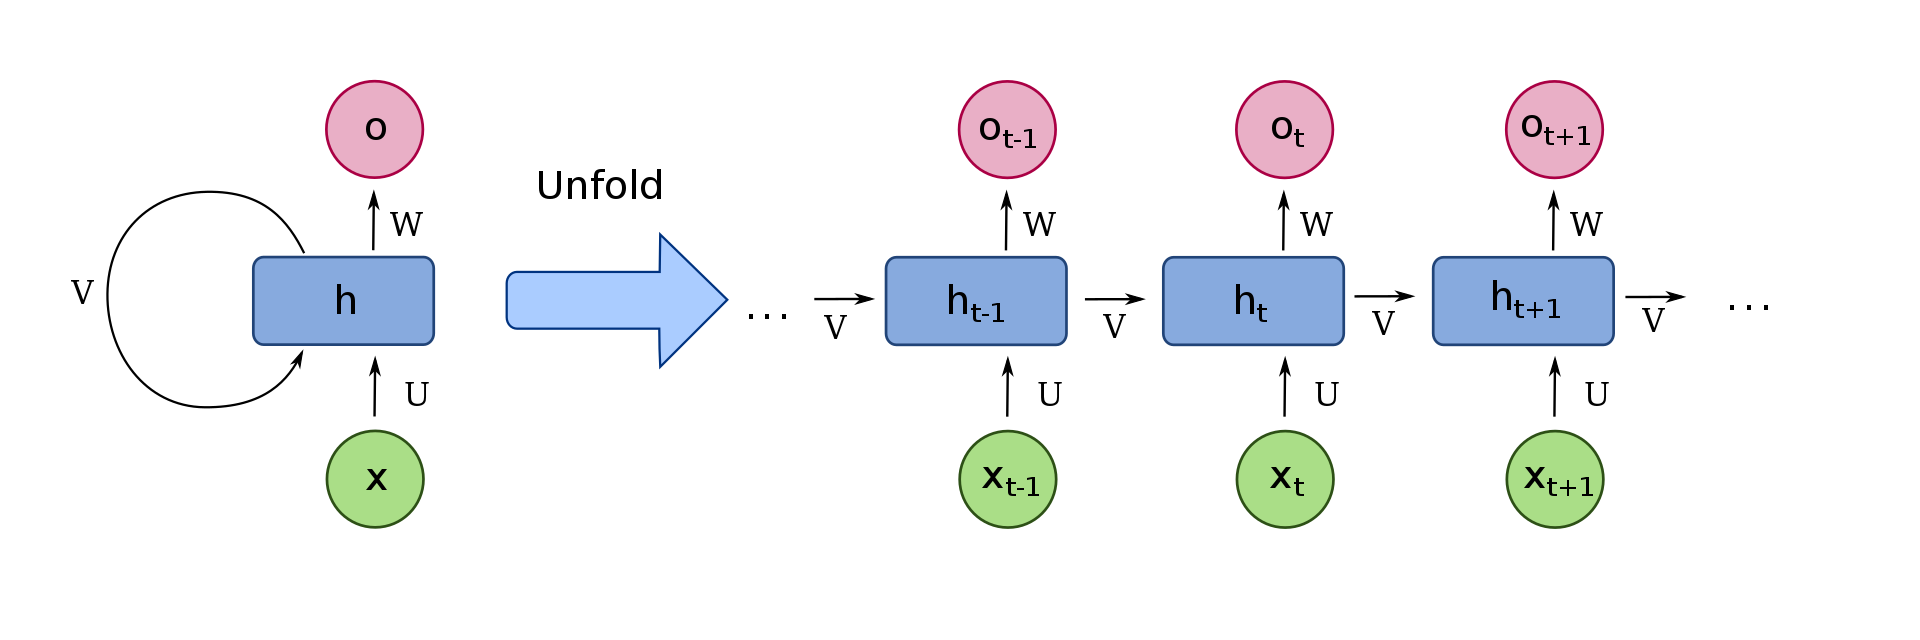
\includegraphics[width=.9\linewidth]{./img/RNN.png}
\caption{folded (left) and unfolded (right) RNN diagram}
\end{figure}


\let\thefootnote\relax\footnotetext{image from https://2d3d.ai/index.php/2019/11/11/the-deep-learning-dictionary/} 

Procedure for training RNNs is called Backpropagation Through Time and is illustrated in the image above.
This works almost like training regular feedforward network, but the parameters of connections for each step are tied.

\begin{enumerate}
\item\relax [TODO???] Problems with RNNs LSTM and Gated Units


\begin{itemize}
\item ELMO, AWD-LSTM?
\end{itemize}
\end{enumerate}

\section{Neural Language Models}

First neural LMs were using RNNs where predicted sequence was shifted to the right (at time \(t\), given \(x_t\) try to predict \(x_{t+1})\)

These models were shown to be useful for various NLP tasks in \emph{Natural Language Processing (Almost) from Scratch} \cite{nlp_scratch} .
Authors used the method to work only using text.
The obtained results were close to previous state-of-the-art approaches that used hand-crafted features,
while using significantly simpler models.

\subsection{Word embeddings}

Training LMs using RNNs requires unrolling which is hard to parallelize.
This makes it time-consuming, and sometimes useful word embeddings might be obtained not using information about whole sequences.

Simpler methods for word embeddings, only making use of fixed-size contexts, were proposed based on \emph{distributional hypothesis}.
They obtain word vectors such that \(vector(w)\) is similar to \(vector(w')\) if \(w\) and \(w'\) occur in similar contexts, for example "Italy" and "France". 

These methods given a sequence  \((w_0, w_{t-1}, w_t, w_{t+1}, ..., w_{T-1})\) try to predict \(w_t\) by the rest of the context.

$$p(w_t, (w_0, w_{t-1}, w_{t+1}, ..., w_{T-1})) = \prod_{i < T, i \neq t} p( w_t|w_i)$$


\begin{enumerate}
\item Word2Vec

This method, proposed in Mikolov et al, 2013 \cite{word2vec} is posed as a standard classification problem and solved using a shallow neural network.

Let us denote by \(W\) the matrix of weights such that \(W(w)\) is the \(w\)'s embedding.

Formally \(p( w_t|w_i) = \frac{e^{W(w_t)^T W(w_i)}}{\sum_k e^{W(w_)^T W(w_k)}}\)

The model is thus trained to minimize
$$\mathcal{L} = -\mathbb{E}_w[log( p(w_t, (w_0, ..., w_{t-1}, w_{t+1}, ..., w_{T-1})))] = $$
$$ = -\mathbb{E}_w[\sum log( p( w_t|w_j)] = \mathbb{E}_w[\sum log(\frac{e^{W(w_t)^T W(w_j)}}{\sum_k e^{W(w_t)^T W(w_k)}} )] = $$
$$ \mathbb{E}_w[\sum W(w_t)^T W(w_j) - T log({\sum_k e^{W(w_t)^T W(w_k)}} )]$$
The weights between input and hidden layer can be then used as word vectors.
Empirically they have been shown that they capture the similarity of words that have similar contexts.
In addition to that it also has been shown that geometry of these word embeddings encodes semantic relations, for example
$$vector("king") - vector("man") \approx vector("queen") - vector("woman")$$

The exact formulation has the problem in that would require \(W_i^T W_k\) for all \(i, j\).
This is unfeasible, as it is \(O(|Vocab|^2)\).

In practice this is circumvented either using \emph{hierarchical softmax} or \emph{negative sampling}.

Negative sampling approximates 
$$ \mathbb{E}_w[\sum W(w_t)^T W(w_j)] \approx  \sum_{(w_t, w_j) \in Pos}log \sigma(W(w_t)^T W(w_j))$$
Where \((w_t, w_j) \in Pos\) means these words occur in some context in data

and

$$ log({\sum_k e^{W(w_t)^T W(w_k)}} ) \approx \sum_{(w_t, w_j) \in Neg} log(\sigma(-W(w_t)^T W(w_j)))$$

where \((w_t, w_j) \in Neg\) are sampled randomly. 

\item FastText

One problem of using words as tokens is that they treat them as atomic units, so either tokens need to be stemmed or lemmatized,
or they will get treated as unrelated.

A series of papers from starting from 
Bojanowski et al, 2017 \cite{fasttext} proposed to refine Word2Vec model with subword information.
These methods split words into tokens, for example "technical" might be split into "techn*" "*ical",
so it will have similar parts with "technician".
Although pretrained language models can be used to extract good representations in context, it remains a 

In our work FastText is useful for embedding Python function names,
as it might figure out that for example "\(get\_http\_request\)" is not an atomic entity.
\end{enumerate}
Although pretrained language models can be used to extract good representations in context, it remains a 

\subsection{[TODO???] Attention and Transformer-based models}

\subsubsection{Sentence embedding models}

Although pretrained language models can be used to extract good representations in context, the representations of whole documents they provide are poor because they need a pooling step to represent a document.

Because of this various methods were proposed to finetune 

There are two most known ways to finetune pretrained transformers for search:

\begin{enumerate}
    \item \textbf{bi-encoders} (also known as dual encoders).
    
    These models are trained by using pairwise similarity of document features. Typically these features are done by feeding texts into transformer models and pooling, so that each document is represented by fixed-length vector. These vectors are compared using a similarity function like cosine similarity which serves as a relevance score.
    
    \item  \textbf{cross-encoders}
    
    In this method a text that is a concatenation of query and relevant document is fed into a transformer model. The model itself outputs relevance score.
\end{enumerate}

In practice cross-encoders tend to give better results. This intuitively makes sense because they can use attention over tokens from query and document. 

Unfortunately cross-encoders have serious drawback, as at search time they require running transformer for each document. Thus cross-encoders mostly remain useful for finetuning tasks. Bi-encoders are used widely because they only require extracting feature from each query, and finding matching documents can be used with vector search engines.

\section{Zero-shot Learning}

Because our queries and features come from possibly different modalities (natural language vs code or its representations) we cannot easily use standard ranking methods for information retrieval.

To circumvent this, and also the fact that we cannot use supervised learning (test queries are not seen in training set) we use zero-shot learning.

Zero-shot Learning (ZSL) is a branch of Machine Learning where classes from test set possibly do not occur in training set.

Because it is impossible to transfer between seen to unseen classes using label encoding or one-hot encoding, to sidestep this ZSL assumes that classes are represented by their feature vectors.

These features might be manually constructed as shown in the following image, or they might consist of NLP-extracted features of class names.

To evaluate ZSL a protocol was proposed in \cite{zsl_good_bad} that takes into account the fact that accuracy on test set will be lower also because the classes were not seen - the authors propose to use harmonic mean of training/validation and test accuracies.

\begin{figure}[htbp]
\centering
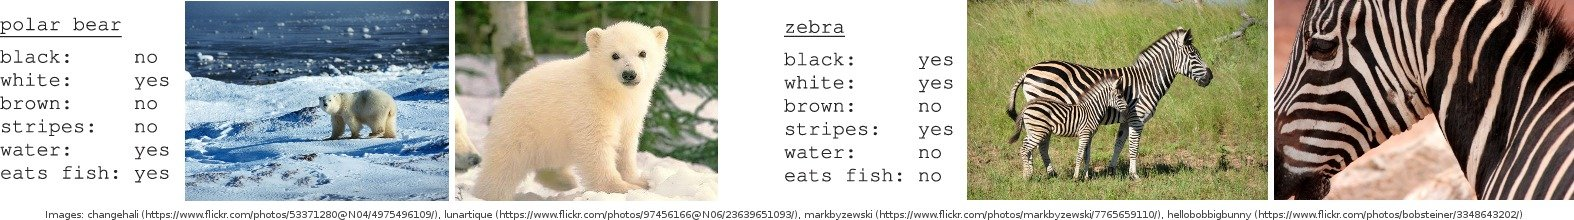
\includegraphics[width=.9\linewidth]{./img/awa2.jpg}
\caption{samples from AWA2 dataset showing images and class features}
\end{figure}

\subsubsection{{\bfseries\sffamily TODO} - ZSL algorithms}


\section{Graphs in Machine Learning}

There exist numerous methods for analyzing graph data that are based on random walks (PageRank, Node2Vec) or graph Laplacian matrix.

Graph Laplacian is defined as $$L = D - A$$ where \(D\) is diagonal matrix where \(D_{ii} = degree(v_i)\), and \(A\) is adjacency matrix.

Methods that use Laplacian matrix, like spectral clustering, typically work by decomposing \(L\), so they can be used for dimensionality reduction.

It is also worth mentioning that many methods for nonlinear dimensionality reduction like Isomap or tSNE also use graphs.
These methods utilize nearest-neighbor graph, in the case of Isomap a distance between points of data manifold is estimated from this graph.

In the following we will focus on Graph Neural Networks (GraphSAGE in particular).

Most older methods for node embeddings are \emph{transductive}, so they assume the same graph structure at training time and test time.
This can be problematic, because it means that models embed every vertex separately, which means that these models have \(O(|V|)\) parameters.
To circumvent this \emph{inductive} models like GraphSAGE were introduced.

\subsubsection{Graph Neural Networks}

Using neural networks for graph-structured data is problematic, because
\begin{itemize}
\item node neighborhoods \(\mathcal{N}(u)\) may vary in size, and NN layers usually assume fixed-size input
\item there is no natural ordering on neighbors
\end{itemize}

First issue is less severe because we might just sample neighbors so that their number becomes fixed in each iteration.
The second one is usually circumvented by explicitly making output layer \emph{permutation invariant} or \emph{equivariant}.

Formally, let us assume that our NN layer \(f\) takes \(A\), graph adjacency matrix as input.

Then $$f(PAP^T) = f(A)$$ means that the layers is \emph{permutation invariant}, whereas  
$$f(PAP^T) = P f(A)$$ means \emph{permutation equivariance}. 

\subsubsection{General framework, message passing}

The general approach for defining GNNs is called \emph{message passing} and can be interpreted as generalization of convolution to graph data or
differentiable graph isomorphism test. The intuition is to incorporate information from neighborhoods so that after each epoch it
propagates through graph.

Formally specifying one layer consists of defining node's \(u\) embedding \(h^{(k+1)}_u\) (superscripts denote layer number).

\(h^{(0)}_u\) are either initialized with some other methods (for example using word embeddings of node names)
or by using graph features (node degree et c).

The embeddings of next layer are then

$$ m_{neigh}(u) = \textsc{aggregate}( \{h^{(k)}_v\}_{v \in \mathcal{N}(u)})$$

$$h^{(k+1)}_u = \textsc{update}(h^{(k)}_u, m_{neigh})$$



where \(\textsc{update}\) and \(\textsc{aggregate}\) are some differentiable functions.

Note that second argument of \(\textsc{update}\) is a set, so this part needs to be permutation invariant.
This can be achieved using functions that don't depend on ordering of the input.
It is usually achieved using pooling functions like averaging or taking maximum, or by averaging method that is order-sensitive (like LSTM encoder) over sample of permutations.

\subsubsection{GNN}
%\begin{equation}
%\tag{basic GNN equation}
%    h^{(k+1)}_u = \sigma(W^{(k)}_{self} h^{(k)}_u + W^{(k)}_{neigh} \sum_{v \in \mathcal{N}(u) h^{(k)}_v})%
%
%\end{equation}

\subsubsection{Scalability, GraphSAGE}

It is easy to come up with vectorized form of GNN equation that takes the whole graph into account to enable whole batch gradient descent:

    $$H^{(k+1)} = \sigma(W^{(k)}_{self} H^{(k)} + A W^{(k)}_{neigh} H^{(k)} + b_k)$$


Where \(A\) is graph's adjacency matrix. The problem with this equation is that it is not easy to turn this into minibatch version.
This is because the second appearance of \(H^{(k)}\) cannot be just replaced by batched version - one would need to
take neighbors into account.

Because of this, several approaches for scaling GNNs were proposed.

One such example is GraphSAGE proposed in Hamilton et al, 2017 \cite{graphsage} It creates minibatches by sampling nodes,
and creating fixed size contexts from their neighbors. 


\begin{figure}[htbp]
\centering
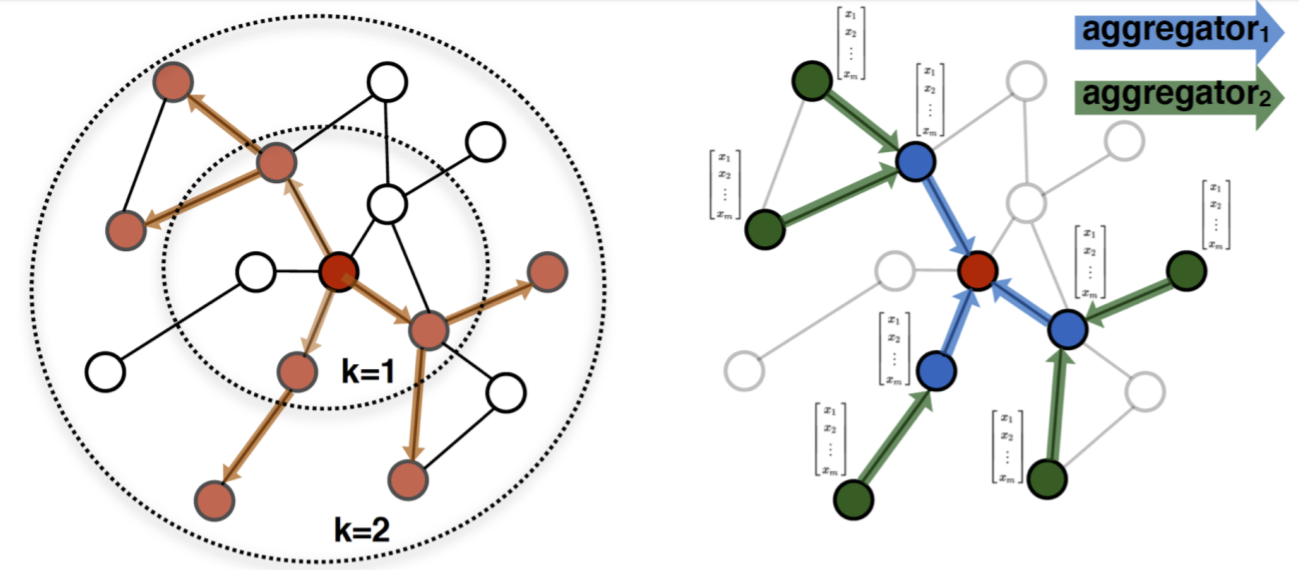
\includegraphics[width=.9\linewidth]{./img/sage_pool.png}
\caption{GraphSAGE: SAmple and AggregatE}
\end{figure}

\let\thefootnote\relax\footnotetext{image from http://snap.stanford.edu/graphsage/} 


Formally, for each minibatch \(B\), \(K\) -layer GraphSAGE fetches embeddings of nodes sampled from \(K\) -hop neighborhoods of each \(u \in B\).

This is achieved by the following algorithm:
\begin{algorithm}[htbp]
\caption{name\ embedding generation (i.e., forward propagation) algorithm}
\label{alg:basic}
	\SetKwInOut{Input}{Input}\SetKwInOut{Output}{Output}
    \Input{~Graph $\G(\V,\E)$; input features $\{\mb{x}_v, \forall v\in \V\}$; depth $K$; weight matrices $\mb{W}^{k}, \forall k \in \{1,...,K\}$; non-linearity $\sigma$; differentiable aggregator functions $\textsc{aggregate}_k, \forall k \in \{1,...,K\}$; neighborhood function $\mathcal{N} : v \rightarrow 2^{\V}$}
    \Output{~Vector representations $\mb{z}_v$ for all $v \in \V$}
    \BlankLine
    $\mb{h}^0_v \leftarrow \mb{x}_v, \forall v \in \V$ \;
    \For{$k=1...K$}{
    	  \For{$v \in \V$}{
    	  $\mb{h}^{k}_{\mathcal{N}(v)} \leftarrow \textsc{aggregate}_k(\{\mb{h}_u^{k-1}, \forall u \in \mathcal{N}(v)\})$\;
    	  		$\mb{h}^k_v \leftarrow \sigma\left(\mb{W}^{k}\cdot\textsc{concat}(\mb{h}_v^{k-1}, \mb{h}^{k}_{\mathcal{N}(v)})\right)$
    	  }
    	  $\mb{h}^{k}_v\leftarrow \mb{h}^{k}_v/ \|\mb{h}^{k}_v\|_2, \forall v \in \V$
    	}
     $\mb{z}_v\leftarrow \mb{h}^{K}_v, \forall v \in \V$ 
\end{algorithm}



\subsubsection{[TODO???] Deep Graph Infomax}
Method related to Masked Language Models


\chapter{Related work}


\section{Mining Software Repositories conference}

Using NLP and more generally machine learning for analyzing code has long history. Mining Software Repositories (MSR) \cite{DBLP:conf/msr/2021} is an example conference on this topic, existing from 2004.

Papers submitted to MSR typically focus on several tasks:
\begin{itemize}
\item software error detection and correction
\item mining software QA sites
\item mining metadata (commit history et c) of sotware projects
\item NLP in software engineering
\end{itemize}

Another research track relevant to our work is using neural networks for feature extraction from code. These features are then used for code classification, generation or search.

\section{Programming languages as machine learning data}

\subsubsection{Code Search}
Code search which is one of the most significant programming activities is not well researched topic. Chao Liu et al \cite{code_search} review papers that try to tackle this problem, and they identify several issues that might explain this relative obscurity. The authors hypothesize that due to lack of standardization and big, clean datasets it is hard to talk about progress in this area. They identify several issues with code search that are typically solved by the papers:

\begin{enumerate}
\label{codesearch}
    \item benchmarks - providing datasets for relevant problems
    \item learning models - coming up with learning metrics, representation methods and new models
    \item model fusion - combining different kinds of models like classical information retrieval and deep learning 
    \item cross-language search - building multi-language tools
    \item search tasks - solving novel search-related problems like searching code from programming video tutorials
\end{enumerate}


\subsection{Tasks}

Code search tasks may be split into categories according to scale of expected results

\begin{center}
\begin{tabular}{|p{2cm}|p{4cm}|p{3cm}|p{4cm}|}
\hline
type & microscopic  & mesoscopic & macroscopic\\
\hline
expected results & code snippet or method & file or bigger code fragment & whole project\\
\hline
example tasks & text-based code snippet search \newline IO based search & clone detection \newline  UI search \newline API search  & find library or project (our problem) \\
\hline
\end{tabular}
\end{center}

\subsection{Performance metrics}

\subsection{Models}

\subsubsection{Code2Vec}

\subsubsection{CodeSearchNet}
Husain et al 2019 \cite{DBLP:journals/corr/abs-1909-09436} propose a dataset for semantic search of code snippets. They use pretrained CodeBert model Feng et al, 2020 \cite{feng2020codebert} which is then trained for matching of function comments with code.
This can be considered as microscopic version of our problem, as we propose to match \textbf{repositories} with descriptions. 

\subsubsection{Import2Vec}

Theeten et al, 2019 \cite{DBLP:journals/corr/abs-1904-03990} explore using Word2Vec model for extracting features of modules. Import2Vec is an unsupervised model which tries to classify whether two modules cooccur in some context.
The approach proposed in this paper is most relevant to our work, as it is the only approach that provides features for higher-level software objects.
Whereas most work focuses on extracting features for code snippets or functions, Import2Vec provides features that can be directly used to featurize repositories.

\subsection{Attention models}

\begin{enumerate}
\item CodeSearchNet

\item CodeBERT

\item{CodeT5}

\end{enumerate}

\subsection{Auxillary techniques}

\subsection{Challenges}

\section{Programming language-specific feature extraction}

In the following we list topics related to our problem and summarize important papers.
The two approaches most relevant for our work are Language Models for code search and Import2Vec.

\section{Hierarchical structure}

Because repository code consists of files, which in turn consist of classes and methods defined in them, a natural question is:

\textbf{\textbf{RQ1: can we leverage this hierarchy to obtain better features?}}

The following work evaluates following approaches to use hierarchical structure of repositories:

\begin{itemize}
\item use definition dependencies (file contains functions, functions contain other subfunctions called in them etc) to create a graph that can be used to extract features
\item summarize repositories using clustering methods
\end{itemize}


\begin{enumerate}
\item Hyperbolic geometry for exploiting hierarchical graph structure


Embeddings of graphs, and more general, finite metric spaces into Euclidean spaces is a well-studied topic.
An example fact about such embeddings is Johnson-Lindenstrauss Lemma.

A known fact about such embeddings is that they have large distortion for some classes of graphs. For example, there doesn't exist an isometric embedding of ternary tree into Euclidean space.

In contrast to this, for each tree there exists an embedding into 2-dimensional hyperbolic space with low distortion, as proved in Sarkar 2011 \cite{sarkar}.

This fact justifies calling hyperbolic spaces continuous analogs of trees.

\begin{enumerate}
\item Hyperbolic graph embeddings

     Embeddings into hyperbolic spaces were first proposed in Poincaré Embeddings for
Learning Hierarchical Representations \cite{poincare}.

Because of numerical issues with Poincare model (in this model hyperbolic space is represented by unit disk, where distances between points near the unit circle are unbounded) there have been proposals for improving this model using hyperboloid (Lorentz) model.

One of these is Hyperbolic Multidimensional Scaling proposed in Representation Tradeoffs for Hyperbolic Embeddings \cite{tradeoffs}.

Comparing these methods is challenging, especially for larger networks, as some of them use distance matrices.

\textbf{\textbf{RQ: are embeddings into hyperbolic spaces feasible for big graphs?}}
\end{enumerate}
\end{enumerate}


\chapter{Data}


\section{Dataset}
\subsection{Sources}



\begin{enumerate}

\item Project README

\item Python function call graph

\end{enumerate}


\subsection{Train-test split}

Test queries were selected as 20\% from each PapersWithCode area.



\section{Data Sources}

\subsection{Raw Data}

\subsubsection{Papers}

We use publicly available Papers with Code dataset \footnote{1 \url{https://github.com/paperswithcode/paperswithcode-data}}

It contains paper title, abstract, and links to both arxiv pdf and github repository.

Dataset contains information about over 50 thousands papers and implementations.

Using this data we can extract paper tasks. Tasks were filtered to remove rare ones that had less than 10 papers. Papers without any task that occured 10 times or more were dropped.

There are TODO \textbf{tasks} that are used for queries. PapersWithCode groups them into areas:

\begin{center}

\begin{tabular}{lr}
\toprule
area & number of tasks  \\
\midrule
\hline
computer-vision             &   107 \\
miscellaneous               &   104 \\
natural-language-processing &    77 \\
methodology                 &    64 \\
graphs                      &    15 \\
medical                     &    14 \\
speech                      &    13 \\
time-series                 &    10 \\
playing-games               &     9 \\
robots                      &     8 \\
audio                       &     6 \\
knowledge-base              &     5 \\
music                       &     5 \\
reasoning                   &     3 \\
computer-code               &     3 \\
adversarial                 &     3 \\
\bottomrule
\end{tabular}

\end{center}

\subsection{Text corpora}



\begin{itemize}

\item paper abstracts (only used in topline)

\item Python code

\item README files

\end{itemize}



\section{Extracted datasets}





\subsection{Python functions}



\begin{center}
\begin{figure}[htbp]
\centering
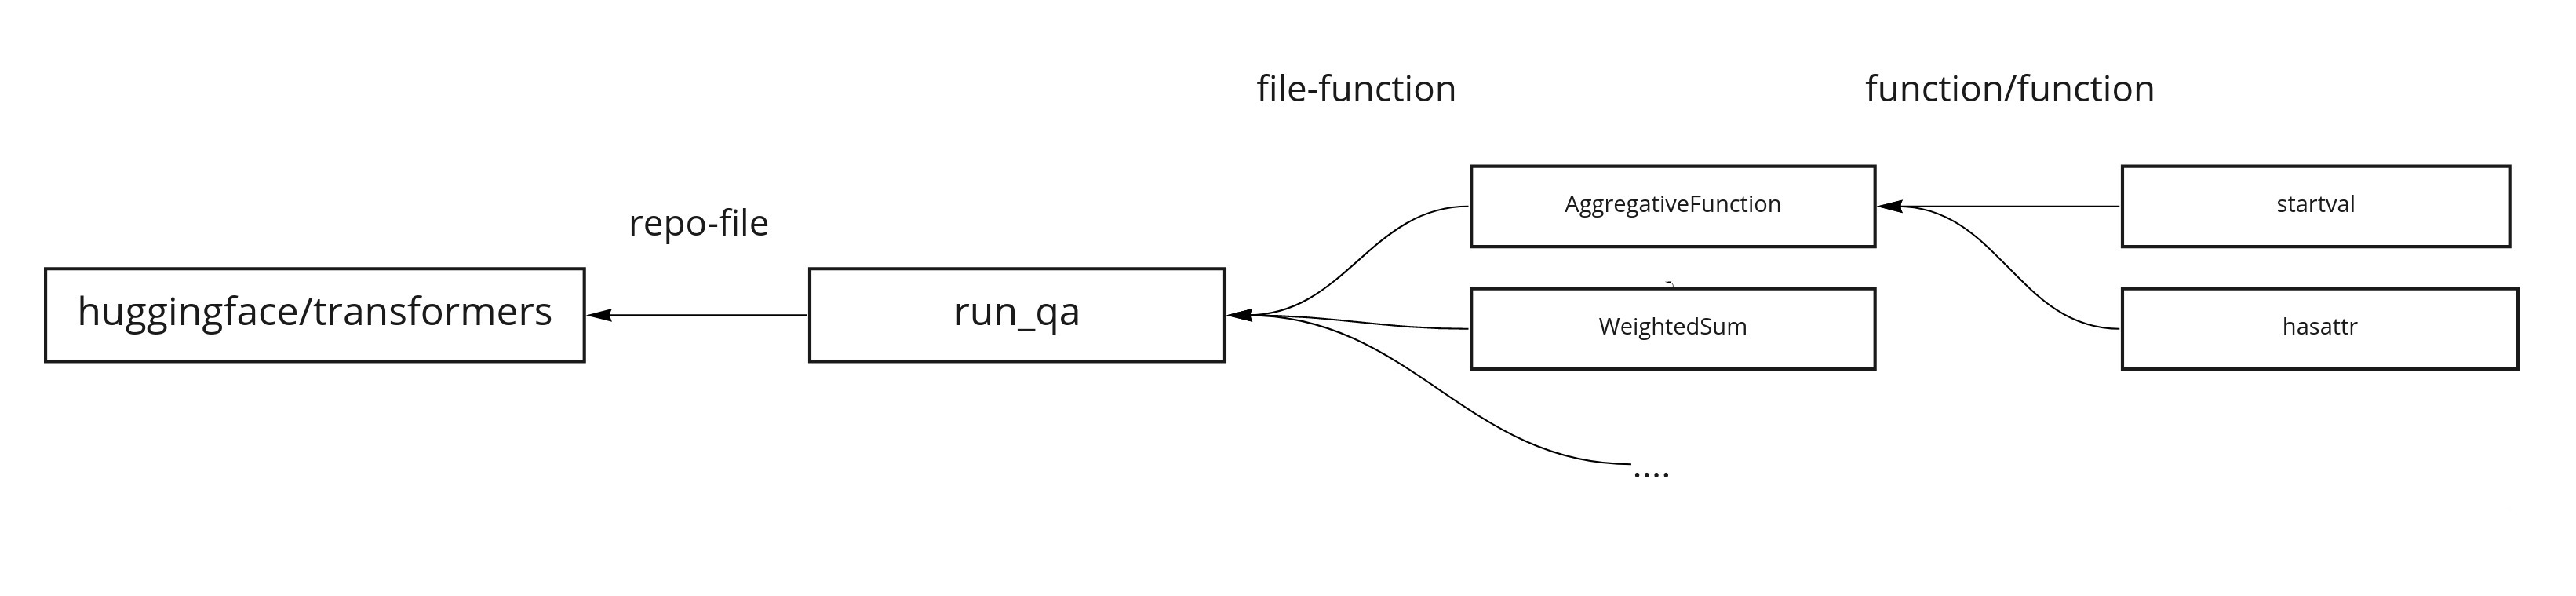
\includegraphics[width=1.25\linewidth]{./img/graph_diagram.jpg}
\caption{example subgraph}
\end{figure}
\end{center}


Using `ast` Python files were parsed and then used to extract class and function definitions.



\subsection{Python Dependency graph}
\label{python-graph}



We define a directed graph  \((V, E)\) where 



\(V_{repo}\) - repository edges



\(V_{file}\) - files from repositorires 



\(V_{df}\) - functions defined in repositories



\(V_{cf}\) - functions called in functions defined in repositories



\(V = \{ROOT\} \cup V_{repo} \cup V_{file} \cup V_{df} \cup V_{cf}\)



Vertices from \(V\) form dependency hierarchy, where next level contains elements dependent on previous level elements.

This gives a natural definition of (directed) edges:

\((v, w) \in E\) if \(w\) is defined/contained in \(v\), where \(v\) is from one level higher (root-repo, repo-file, file-function, function-called function)

\chapter{Approach}

\section{Introduction}

As a proxy for retrieval by natural language queries we  evaluate retrieval of arXiv paper's Python repository given its PapersWithCode \textbf{task}.


\begin{table}[hbt!]
\caption{Gold standard results for 'anomaly detection' task}
\begin{tabular}{|p{6cm}|c|}
\hline                                                                                                                paper title &                                repository name\\ \hline
\midrule
                                                                PyOD: A Python Toolbox for Scalable Outlier Detection &                      winstonll/SynC \\ \hline
 Anomalous Sound Detection as a Simple Binary Classification Problem with Careful Selection of Proxy Outlier Examples &    OptimusPrimus/dcase2020\_workshop \\ \hline
                                                               Learning Generalized Spoof Cues for Face Anti-spoofing &     Podidiving/lgsc-for-fas-pytorch \\ \hline
                                                                Combining Machine Learning Models using combo Library &                      yzhao062/combo \\ \hline
                                        Detecting Regions of Maximal Divergence for Spatio-Temporal Anomaly Detection &                    cvjena/libmaxdiv \\ \hline
\end{tabular}
\end{table}

\newpage 
We propose to tackle this information retrieval problem using progressively
relaxed  
assumptions: 

\begin{itemize}
\item repository is described by paper abstract
\item repository has a README file
\item repository has none of the above 
\end{itemize}

Each step of this hierarchy corresponds growing usefulness of the system. In
general we cannot assume that a repository will easily match any paper, and
dropping README requirement might be helpful as it might make useful code
accessible even before authors decide to summarize their work. 

\section{General ideas}

\subsection{Feature extraction and zero-shot learning}
\subsubsection{TODO schematic}

Our system can be decomposed into two separate parts:

\begin{enumerate}

\item Repository feature extraction

\item Matching repository features with query features

\end{enumerate}

\subsubsection{Matching queries with repositories}

We use Zero-shot learning (ZSL) methods because there is a need to match representations from different domains,

for example FastText vectors for query and graph-based representation of repository.

Existing Zero-shot learning methods typically model similarity between entities that use different representations.

This naturally fits our problem as most information retrieval models use query-document similarities to find most relevant documents.

\subsubsection{Query features}

Because ZSL needs class features, we evaluate several methods for extracting representations from PapersWithCode task names:
\begin{itemize}
\item pretrained word embeddings available in Gensim \cite{rehurek2011gensim}
\item word embeddings (FastText and Word2Vec) trained on Python file corpus
\end{itemize}

\subsubsection{Repository features}

    Due to explosion of interest in transformer-based models in NLP there exist several methods enabling search beyond bag-of-words model.

    This kind of functionality is very useful for cases where given specific query we want to find text fragment related to query, like in question answering models

Unfortunately this cannot be used as-is for repository search, because repositories contain multitude of such fragments.

This means that for repository search we would need to find method  for extracting features from parts into more global features.

We use several methods to extract repository features
\begin{itemize}
    \item text features extracted from README. These use either FastText or Word2Vec.
    \item Import2Vec features
    \item graph Node Embedding features (these methods are inductive, so the main point of using them is to compare their results to GNN features)
    \item GNN features extracted using GraphSAGE
\end{itemize}


\subsection{Proxy ZSL problem}


Zero-shot learning algorithms are used for matching task \(\phi(t)\) features with repository \(\psi(r)\) features. Using these features ZSL model comes up with a scoring function $F(t, r)$ that measures how well repository $r$ matches task $t$.

For simplicity we only use single-label Zero-Shot learning methods. For this we needed to extract single task that best describes the repository. One way to do this is to select \textbf{least common task}.

Using \(F(t, r)\) learned with ZSL methods we score task-repository similarities and for a given repository retrieve top \(k\) matched tasks.

\subsection{Sentence embeddings}

Using sentence transformers we can finetune models that are trained for various tasks like comment generation or summarization to extract features for whole texts.

\paragraph{Used datasets}

\subsection{Sequence-to-sequence models}

Language models pretrained on various code tasks can be used to extract shorter versions (like summaries) that can be used for
\begin{itemize}
    \item query expansion
    \item document representations for better sentence embeddings
\end{itemize}


\paragraph{README summarization}

\paragraph{Code summarization}

\subsubsection{Information retrieval as sequence-to-sequence task}

We adapt approach from Differentiable Search Index \cite{differentiable_search_index} paper for information retrieval using sequence2sequence models.

TODO: low compute

Because code dataset is naturally hierarchicaly structured, we try to use file paths analogously to semantic document IDs from \cite{differentiable_search_index}.

\textbf{pegasus <REPO SEP> pegasus/models/transformer.py 
}

TODO: better example 

TODO: special tokens

\section{Representation}

\begin{enumerate}

\item Text data:

\begin{enumerate}

\item Word2Vec

\item FastText

\item Transformer-based features

\item Import2Vec

\end{enumerate}



\item Dependency graph:

\begin{enumerate}

\item Node embeddings

\item GraphSAGE

\end{enumerate}



Graph-based features are extracted for nodes in dependency graph, so for each repository we need to aggregate them from its constituents.

To do this we fetch file name node embeddings, and their average is taken to represent a project.

For transductive models like GraphSAGE we initialize node embeddings with text features (extracted from file names, functions et c).

These representations use either FastText trained on Python code corpus or embeddings CodeBERT model.

\end{enumerate}




\chapter{Evaluation}
\section{Metrics}

We envision two search scenarios:

\begin{enumerate}
    \item Looking for a single or a few relevant projects from a given domain
    \item Browsing projects.
\end{enumerate}

In 1st scenario user is interested to retrieve at least one relevant project. Thus accuracy @ k is appropriate metric.

The 2nd case developer will be interested in having as many relevant projects as high as possible in result list. This can be captured using MAP (mean average precision).


\section{Topline}


Topline was established by matching queries (tasks) with paper abstracts.

\section{Results}
  
 \begin{center}
 \begin{tabular}{ |p{3cm}|p{2cm}|p{2cm}|p{2cm}|}
 \hline
  Repository \newline representation & Query \newline embedding model &  Repository embedding model & Top-10 \newline accuracy \\
 \hline 
  Abstract (topline)                 & Word2Vec              & Word2Vec                   &        \textit{0.828} \\
  README                    & Word2Vec              & Word2Vec                   &            \textbf{0.687} \\
  README                    & Word2Vec              & FastText                   &           0.466 \\
  Imports                   & Word2Vec              & Import2Vec                 &        0.206 \\
  Graph                     & Word2Vec              & ProNE                      &            0.100 \\
  Graph                     & Word2Vec              & GraphSAGE                            & 0.244         \\
 \hline
 \end{tabular}
 \end{center}

\section{Detailed results}

More detailed results are shown that take into account not only literal task match, but also how many papers from related tasks (tasks from the same area as query) were retrieved. We also provide information about relative positions of recalled papers.

\begin{center}
\begin{tabular}{p{1cm}rrrrrr}
\toprule
{} & recalled & num\_recalled & area\_recalled & num\_area\_recalled & area\_recalled\_position & count \\
{} &     mean &         mean &          mean &              mean & \multicolumn{2}{l}{median} \\
area                        &          &              &               &                   &                        &       \\
\midrule
miscellaneous               &     0.45 &         1.17 &          0.91 &              0.91 &                    3.0 &   133 \\
computer-vision             &     0.48 &         1.46 &          0.97 &              0.97 &                    0.0 &   123 \\
methodology                 &     0.56 &         1.26 &          1.00 &              1.00 &                    1.0 &    77 \\
natural-language-processing &     0.31 &         0.81 &          0.92 &              0.92 &                    3.0 &    74 \\
graphs                      &     0.47 &         1.59 &          0.82 &              0.82 &                    1.0 &    17 \\
medical                     &     0.41 &         0.82 &          0.88 &              0.88 &                    2.0 &    17 \\
playing-games               &     0.44 &         1.19 &          0.81 &              0.81 &                    2.5 &    16 \\
speech                      &     0.75 &         1.25 &          0.92 &              0.92 &                    4.0 &    12 \\
time-series                 &     0.45 &         1.09 &          0.82 &              0.82 &                    6.0 &    11 \\
robots                      &     0.30 &         0.70 &          0.50 &              0.50 &                    inf &    10 \\
audio                       &     0.33 &         0.50 &          0.67 &              0.67 &                    0.0 &     6 \\
computer-code               &     0.25 &         0.25 &          0.25 &              0.25 &                    inf &     4 \\
knowledge-base              &     1.00 &         2.00 &          1.00 &              1.00 &                    2.0 &     4 \\
music                       &     0.50 &         0.50 &          0.50 &              0.50 &                    inf &     4 \\
adversarial                 &     1.00 &         2.33 &          1.00 &              1.00 &                    0.0 &     3 \\
reasoning                   &     0.00 &         0.00 &          0.00 &              0.00 &                    inf &     2 \\
\bottomrule
\end{tabular}
\end{center}

\nocite{*}
\bibliographystyle{plain}
\bibliography{refs.bib}


\end{document}
